\documentclass{article}

\usepackage{arxiv}

\usepackage[utf8]{inputenc} % allow utf-8 input
\usepackage[T1]{fontenc}    % use 8-bit T1 fonts
\usepackage{url}            % simple URL typesetting
\usepackage{booktabs}       % professional-quality tables
\usepackage{amsfonts}       % blackboard math symbols
\usepackage{nicefrac}       % compact symbols for 1/2, etc.
\usepackage{microtype}      % microtypography
\usepackage{lipsum}
\usepackage{graphicx}
\usepackage{amsmath}
\usepackage[colorlinks=true, allcolors=blue]{hyperref}

\graphicspath{ {./images/} }


\usepackage[rightcaption]{sidecap}
\usepackage{wrapfig}

% % clean citations
\usepackage{cite}
% % hyperref makes references clicky. use \url{www.example.com} or \href{www.example.com}{description} to add a clicky url
\usepackage{nameref}
% % line numbers
\usepackage[right]{lineno}


\title{Project report \\ Improving Explorability in Variational Inference with Annealed Variational Objectives}
\author{Mikhail Kurenkov, Timur Chikichev, Aleksei Pronkin}
\date{23 October 2020}

\begin{document}
\vspace*{0.35in}

\begin{flushleft}
{\Large
\textbf\newline{Project report \\ Improving Explorability in Variational Inference with Annealed Variational Objectives.}
}
\newline
\\
{Mikhail Kurenkov,
Timur Chikichev,
Aleksei Pronkin}
\\
\bigskip
% * aleksei.pronkin@skoltech.ru
* \url{https://github.com/alexey-pronkin/annealed}

\end{flushleft}

\section*{Abstract}

We represent the results of paper \cite{main_Huang2018ImprovingEI}.
The main work of research is a special procedure, applied into the training of hierarchical variational methods. The method called Annealed Variational Objectives (AVO) has to solve the problem of limited posterior distribution density. The method facilitates learning by integrating energy tempering into the optimization objective.

The paper presents contains experiments on the proposed method. These experiments represent the drawbacks of biasing the true posterior to be unimodal, and show how proposed method solve this problem.
We repeat experiments from \cite{main_Huang2018ImprovingEI} and compare performance of AVO with normalizing flows (NF) and variational auto-encoders (VAE). Additionally we make experiments with deterministic warm up (analogously to AVO), which when applied to NF and VAE may benefits in better space exploration.

% \linenumbers

\section{Introduction}

% related work

% Variational Inference(VI) has played an important role in Bayesian model uncertainty calibration andin unsupervised representation learning. It is different fromMarkov Chain Monte Carlo(MCMC)methods, which rely on the Markov chain to reach an equilibrium; in VI one can easily draw i.i.d.samples from the variational distribution, and enjoy lower variance in inference. On the other handVI is subject to bias on account of the introduction of the approximating variational distribution.As pointed out by Turner and Sahani (2011),  variational approximations tend not to propagateuncertainty well. This inaccuracy and overconfidence in inference can result in bias in statistics ofcertain features of the unobserved variable, such as marginal likelihood of data or the predictiveposterior in the context of a Bayesian model. We argue that this is especially true in the amortized VIsetups (Kingma and Welling, 2014; Rezende et al., 2014), where one seeks to learn the representationsof the data in an efficient manner.  We note that this sacrifices the chance of exploring differentconfigurations of representation in inference, and can bias and hurt the training of the model.This bias is believed to be caused by the variational family that is used, such as factorial Gaussian forcomputational tractability, which limits theexpressivenessof the approximate posterior. In principle,this can be alleviated by having a more rich family of distributions, but in practice, it remains achallenging issue for optimization.  To see this, we write the training objective of VI as the KLdivergence, also known as the variational free energyF, between the proposalqand the target

With variational inference, we have some variational distribution we may use to generate samples. The resulting variance can be lowered by two ways, increasing number of samples and increasing approximation accuracy.
If variational inference has bad uncertainty approximation (Turner and Sahani (2011)), we will receive bias in statistics in terms of overconfidence and inaccuracy. 
The statistics we check in models are marginal likelihood of data and the predictive posterior. 
The same in the amortized VI setups, the representation of data will require better exploration from approximation model during training.

To express the bias induced by a non-rich and non-expressive variational family, the objective can be written as KL-divergence between proposal and target distributions.

Variational inference objective:
\begin{equation*}
    F(q) = E_q[\log q(z) - \log f(z)] = D_{KL}(q\|f)
\end{equation*}

% The question here is how to inhibit the variational approximation from escaping poor local minima, even when it has sufficient

Due to KL-divergence, the resulting approximation will have low probability mass in regions with low density. The variational approximation may escape points with sufficient statistics in true target, but with small local density. For multi-modal target distributions, not all target space will be covered and the model will loose some sufficient statistics.

Annealing techniques may increase exploration of the target density.

Alpha-annealing (expressiveness):

\begin{equation*}
    E_q[\log q(z) - \alpha \log f(z)]
\end{equation*}

where $\alpha \sim \frac{1}{T}$, and $T$ is temperature which defines the speed of approximate model changes, e.g. learning rate. 
When $\alpha$ goes from zero to 1, we obtain the usual objective, but with full energy landscape covered. 

The problem, with low penalty on the energy term, the whole procedure is time consuming. This is because multiple inferences are required on each maximization step (deep neural networks, hierarchical models, etc.).

Beta-annealing (optimization): 

Deterministic warm-up (Raiko et al., 2007) is applied to improve training of a generative model. 
\begin{align*}
    p(x, z) = p(x|z)p(z)
\end{align*}

The joint likelihood is equal to the un-normalized true posterior $f(z) = p(z | x)$.

The annealed objective is (negative ELBO):
\begin{equation*}
    E_q[\beta (\log q(z) - \log p(z)) - \log p(x|z)]
\end{equation*}

In annealed objective, the $\beta$ is annealed from 0 to 1. This disables the regularisation of posterior to be like a prior. First  training the negative log-likelihood, we train the decoder independently. With this the model is trained to fit the data, so we have more deterministic auto-encoder. With this approach we additionally lose in latent space exploration.

% \subsection*{Related work}

The model:
Latent variable model with a joint probability $ p_{\theta}(x, z) = p(x|z)p(z)$.

$x$ and $z$ are observed and latent variables, $\theta$ - model parameters to be learned.

Training procedure, given expected complete data log likelihood over $q$:

\begin{align*}
    \max_{\theta}E_{q(z)} [\log p_{\theta}(x, z)]
\end{align*}

\textbf{Conditional $q(z|x)$}
\begin{enumerate}{}
    \item tractable: Expectation-Maximization(EM) algorithm.
    \item non-tractable: approximate the true posterior (MCMC, VI)
\end{enumerate}

% That is to say, maximizing ECLL increases the marginal likelihood of the data while biasing the true posterior to be more like the auxiliary distribution.  The second effect vanishes when q(z)approximate sp(z|x)better.



\textbf{Variational distribution subfamilies with expressive parametric form}
\begin{enumerate}
    \item Hierarchical Variational Inference(HVI) 
    \item Auxiliary variable methods
    \item Normalizing flows
\end{enumerate}

In HVI, we use a latent variable model $q(z_T) = \int q(z_T, z_{t<T}) d z_{t < T} $, where $t < T$ denoting latent variables.

We use reverse network $r(z_{t < T} )$ to lower bound intractable $q(z_T)$.

\begin{align*}
    &- E_{q(z_T)}[\log q(z_T)] \ge -E_{q(z_T)}[\ 
    \log q(z_T) + D_{KL}(q(z_{t<T} | z_T) || r(z_{t<T} | z_T))] = \\
    &= -E_{q(z_T, z_{t<T})}[\ 
    \log q(z_T | z_{t<T}) q(z_{t<T}) - \log r(z_{t<T} | z_T) ]
\end{align*}

The variational lower bound is:
\begin{align*}
    L(x) = E_{q(z_T, z_{t<T})}[\ 
    \log \frac{p(x, z_T) r(z_{t<T} | z_T)}{q(z_T | z_{t<T}) q(z_{t<T})} ]
\end{align*}

As the $q(z)$ is one from chosen distribution subfamilies, we have the capability to represent any posterior distribution.
If possible to invert $q(z_T | z_{t<T})$, we choose $r$ to be its invert transformation. This is the so called inverse auto-regressive flow (IAF). The KL term is zero, the variance is lower, the entropy is computed via change of the volume formula.

\begin{equation}
    q(z_T) = q(z_{T-1}) |\frac{\partial z_T}{\partial z_{T-1}}|^{-1}
\end{equation}

\subsection*{Loss function tempering: annealed importance sampling}

Annealed importance sampling(AIS) is an MCMC method with same concept as alpha annealing, it let the variational distribution be more exploratory early on during training.

We have an extended state space with $z_0, ..,. z_T$ latent variables.
$z_0$ is sampled from simple distribution (Gaussian normal prior distribution $p(z)$).
Particles are sequentially sampled from the transition operators $q_t(z_t\|z_{t-1})$.

To define transition operators, we design a set of intermediate target densities as 
$\tilde{f_t} = \tilde{f_T^{\alpha_t}}\tilde{f_T^{1 - \alpha_t}}$.
This is the set of targets defined as a mixture of initial (normal) and target (complex multi-modal) distributions.

For intermediate targets to be invariant, the transitions are constructed as Markov chain with the following weights:
\begin{equation*}
    w_j = \frac{\tilde{f_1}(z_1)\tilde{f_2}(z_2)}{\tilde{f_0}(z_1)\tilde{f_1}(z_2)} ... \frac{\tilde{f_T}(z_T)}{\tilde{f_{T-1}}(z_{T})}
\end{equation*}

% A downside of AIS is that it requires constructing 
For the estimate to be accurate we need a long sequence of transitions, computationally difficult.

\subsection*{Annealed Variational Objectives(AVO)}

Similar to AIS and alpha-annealing, authors of \cite{main_Huang2018ImprovingEI} propose to integrate energy tempering into the optimization objective of the variational distribution. 

As in AIS, we consider an extended state space with same transitional targets.
The marginal $q_T(z_T)$ is an approximate posterior. 
To define incremental steps, we construct T forward transition operators and T backward operators. 
We construct intermediate targets
as an interpolation between the true (unnormalized) posterior and the initial (normal) distribution:
$\tilde{f_t} = \tilde{f_T^{\alpha_t}}\tilde{f_T^{1 - \alpha_t}}$, where $\alpha \in [0, 1]$. 



Different from AIS, we learn the parametric transition operators which are assigned to each transition pair. We have a sequence of one layer networks as a result.

Annealed Variational Objectives(AVO):
\begin{align*}
    \max_{q_t(z_t| z_{t-1})r_{t}(z_{t-1} | z_t)} E_{q_t(z_t| z_{t-1})q_{t-1}(z_{t-1})}[\ 
    \log \frac{\tilde{f_t}(z_T) r_{t}(z_{t-1} | z_t)}{q_t(z_t| z_{t-1})q_{t-1}(z_{t-1})} ]
\end{align*}

In implementation we use detach method of the Pytorch for optimization of the AVO loss respect to parameters of $q(z_t|z_{t -1 })$ and $r(z_t|z_{t - 1})$ with fixed $z_{t - 1}$ and $q_{t - 1}(z_{t - 1})$.

Stochastic refinement transition operator:
\begin{align*}
    & q_t(z_t | z_{t - 1}) = N(z_t | \mu_t^q(z_{t - 1}), \sigma_t^q(z_{t - 1})); \\
    & r_t(z_{t - 1} | z_t) = N(z_{t - 1} | \mu_t^r(z_{t}), \sigma_t^r(z_{t})); \\
    & \mu(z) = g(z) \cdot m(z) + (1 - g(z)) \cdot z; \sigma(z) = act_{\sigma}(W_{\sigma}\cdot h(z) + b_{\sigma}) \\
    & m(z) = W_{m}\cdot h(z) + b_{m}; g(z) = act_{g}(W_{g}\cdot h(z) + b_{g}); h(z) = act_{h}(W_{h}\cdot z + b_{h})
\end{align*}

In implementation we use reparametrization technique for performing forward and reverse transitions.

\begin{figure}
    \caption{Annealed Variational Objectives. Transitional targets presented on a first three toy energy functions.}
    \centering
    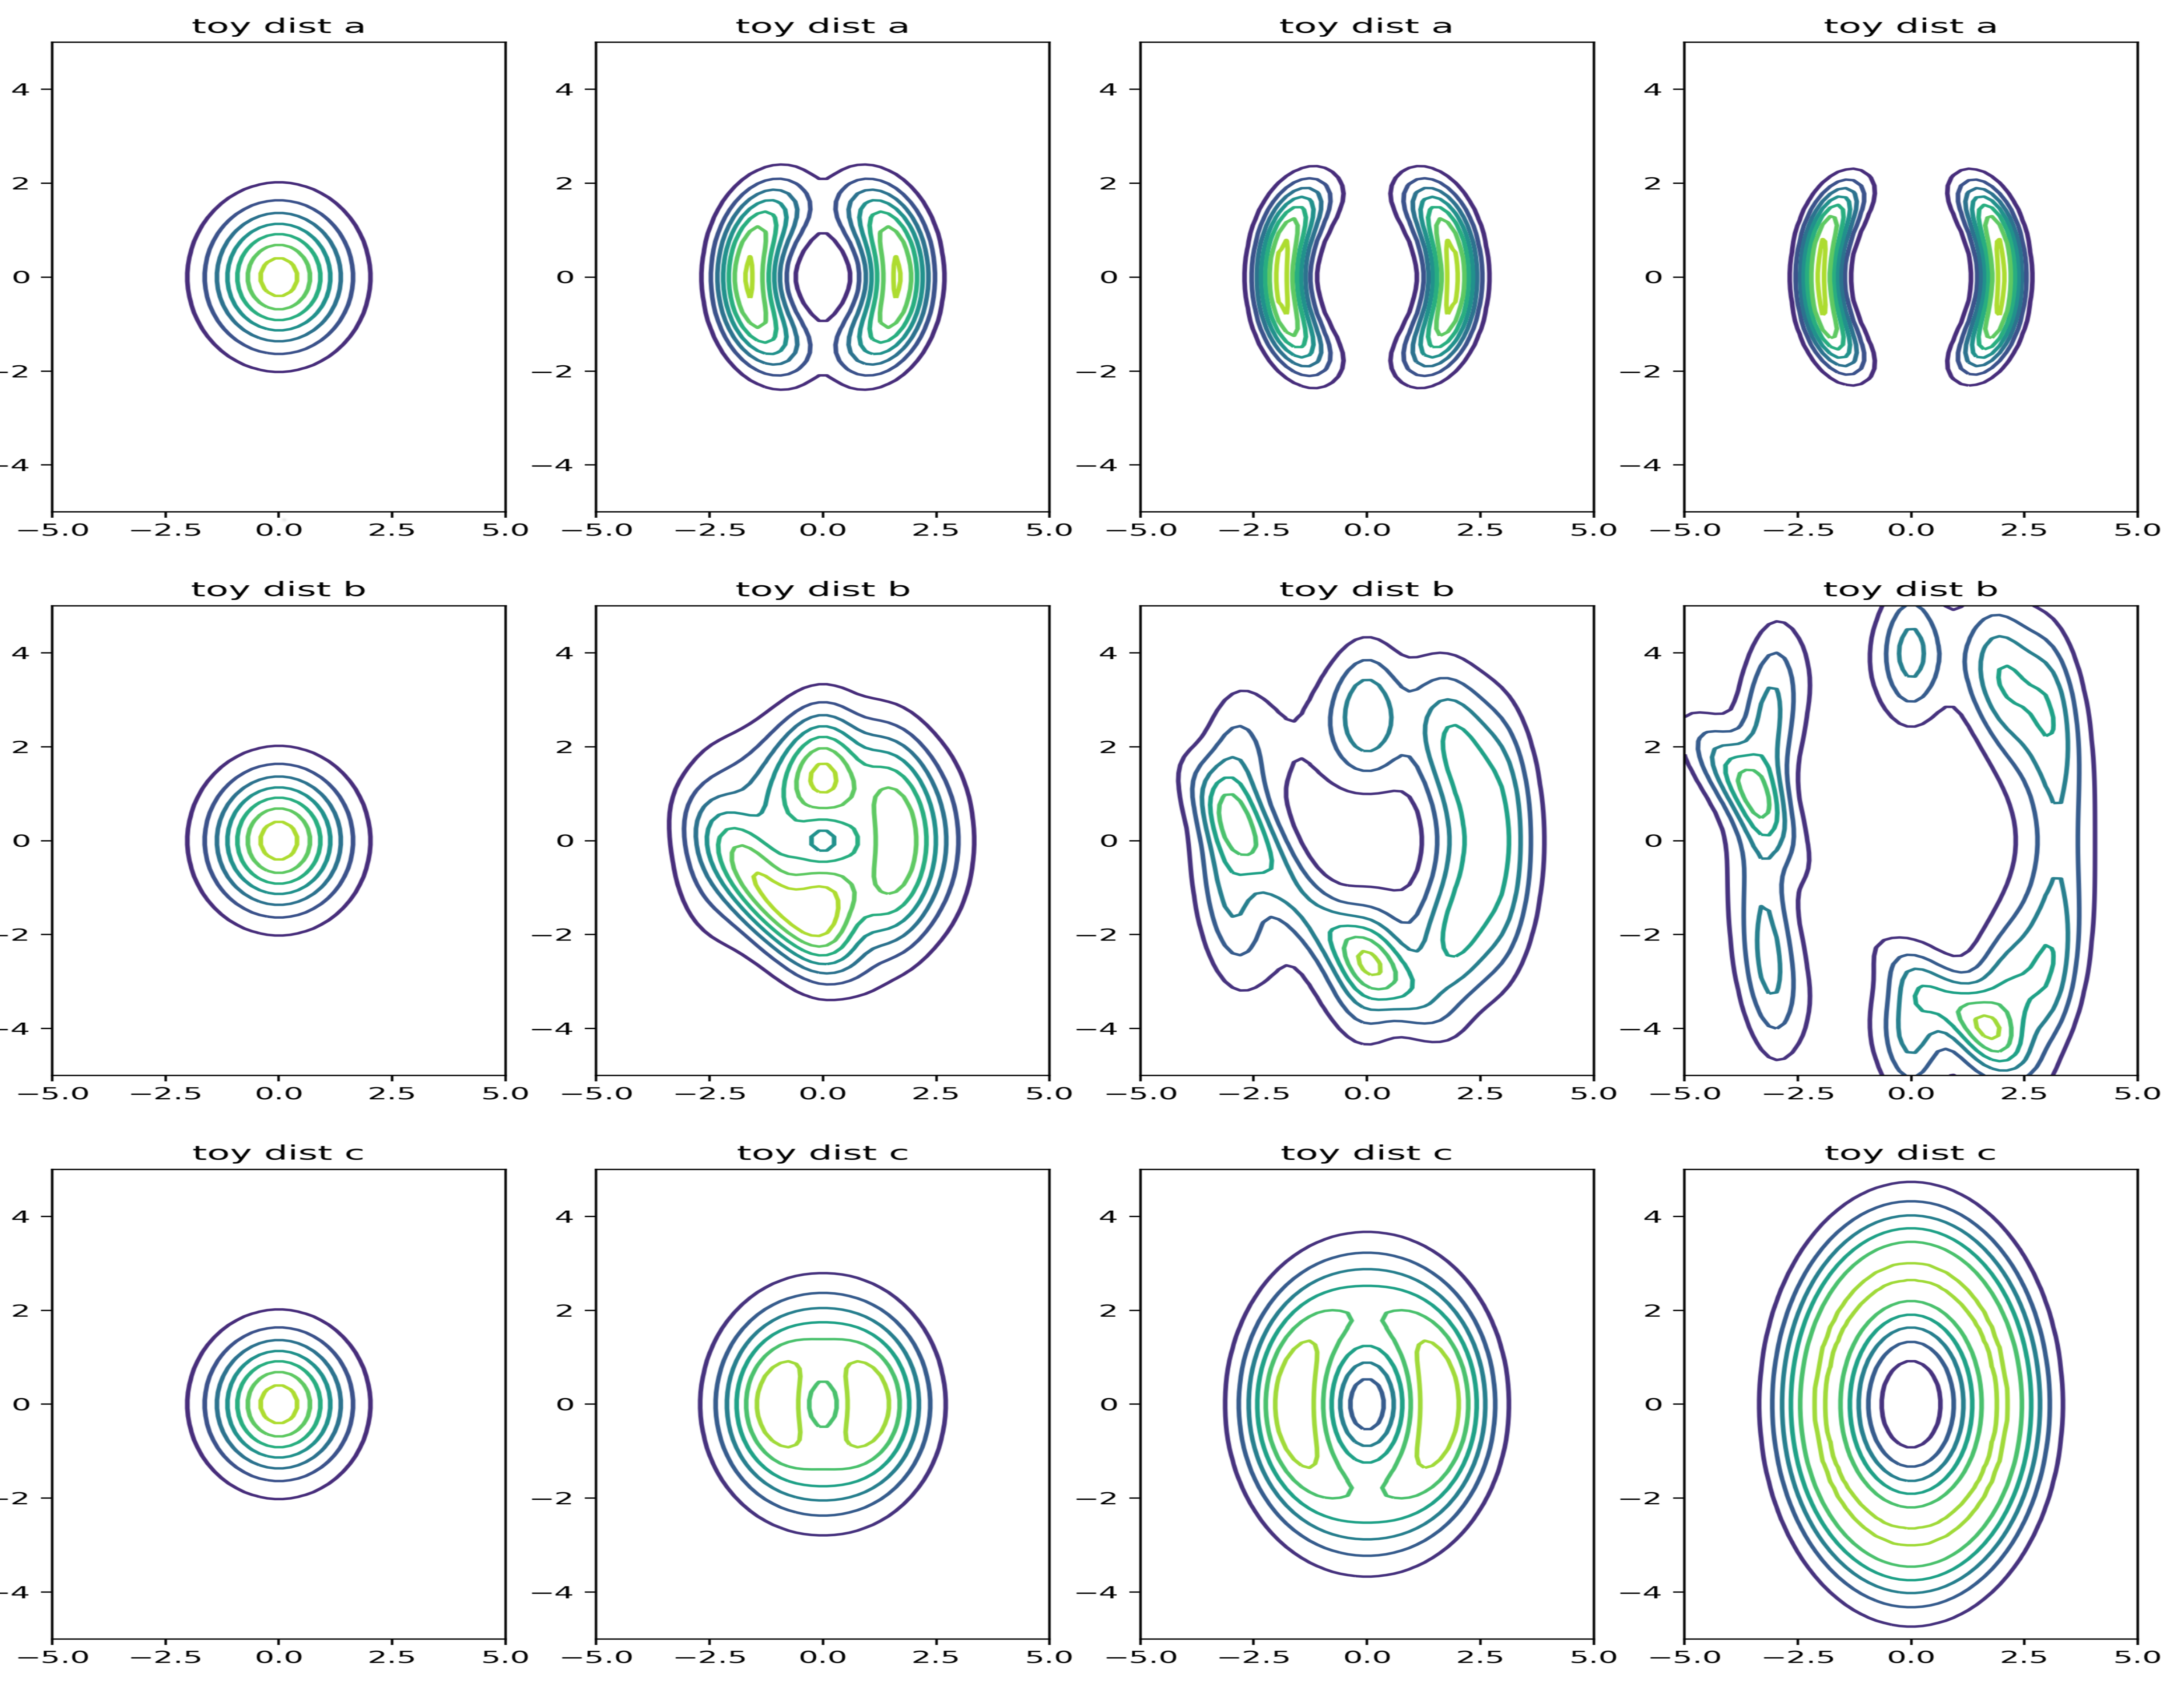
\includegraphics[width=\textwidth]{transitions_targets_abc}
    \label{toyabctrans}
\end{figure}

On figure \ref{toyabctrans}, we present a transitional targets for a first three toy energy functions. The list of all functions used in paper will be presented in section \ref{sec:ToyFit}.


% \begin{figure}
    
% \end{figure}


% Variational Inference ~ reducing representational bias ~ amortized VI, Variational Auto-encoders (VAE)
% Expressive families of variational distributions >> losing the computational tractability
% Reducing the amortization error introduced by the use of a conditional network
% Non-parametric methods
% Importance Weighted Auto-encoder (IWAE) >> multiple samples >> computationally difficult


% Experiments:
% \begin{enumerate}
%     \item Biased noise model.
%     \item Toy energy fitting.
%     \item Quantitative analysis on robustness to beta annealing.
%     \item Amortized inference on MNIST and CelebA datasets.
% \end{enumerate}

% We also want to demonstrate posterior collapse on toy example and show how method from AVO \cite{main_Huang2018ImprovingEI} can mitigate this problem. Also we want to check if Variational Auto Encoder (VAE) can be improved by the AVO method on the MNIST dataset.

% \subsection*{General plan}
% \begin{enumerate}
%     \item Re-implement Variational-Auto Encoder (VAE) \cite{kingma2013autoencoding} with parameters from \cite{TW:2016}. %\url{https://github.com/jmtomczak/vae_householder_flow}
%     \item Implement Hierarchical Variational Model (HVM) based on \cite{ranganath2015hierarchical}.
%     \item Implement Importance Weighted Auto-Encoder (IWAE) based on \cite{burda2015importance}.
%     \item Implement Hierarchical Variational Inference (HVI) method  based on \cite{ranganath2015hierarchical}.
%     \item Implement Annealed Variational Objectives (AVO) method \cite{main_Huang2018ImprovingEI}.
%     \item Analyze a behavior AVO method on toy examples.
%     \item Conduct experiments with VAE and AVO on the MNIST and CelebA datasets.
% \end{enumerate}

\section{Experiments}

\subsection{Toy energy fitting}
\label{sec:ToyFit}


Specification of the toy energy functions:
\begin{align*} \label{toy_models}
&(a) -\frac{((\|z\|_2 - 2) / 0.4)^2}{2} + \
\log(\exp (-\frac{((z_1 - 2) / 0.6)^2}{2}) + \exp (-\frac{((z_1 + 2) / 0.6)^2}{2})) \\
&(b) -\frac{((\|0.5 z\|_2 - 2) / 0.5)^2}{2} + \
\log(\exp (-\frac{((z_1 - 2) / 0.6)^2}{2}) + \exp (-\frac{(2 \sin{z_1})^2}{2}) + \
\exp (-\frac{((z_1 z_2 + 2.5) / 0.6)^2}{2})) \\
&(c) -(2 - \sqrt{z_1^2 + \frac{z_2^2}{2}})^2\\
&(d) \log(0.1 N([-2, 0]^T, 0.2 I) + 0.3 N([2, 0]^T, 0.2 I) + \
0.4 N([0, 2]^T, 0.2 I) + 0.2 N([0, -2]^T, 0.2 I) ) \\
&(e) -\frac{((z_2 - w_1) / 0.4)^2}{2} + 0.1 (z_1^2) \\
&(f) \log(\exp (-\frac{((z_2 - w_1) / 0.35)^2}{2}) + \exp (-\frac{((z_2 - w_1 + w_2) / 0.35)^2}{2})) - 0.05 z_1^2 \\
& w_1 = \sin(\frac{\pi}{2}z_1), w_1 = 3\exp(\frac{(z_1 - 2)^2}{2})
\end{align*}

% \begin{figure}
%     \caption{HVI - AVO, toy energy fitting: target is four-mode mixture of Gaussian}
%     \centering
%     \includegraphics[width=\textwidth]{HVI - AVO}
%     \label{HVIAVO}
% \end{figure}

\subsection{Compare HVI - ELBO and HVI - AVO}

We use HVI with 4 layers (hidden dimension 32, activation - ReLU) ~2k learning parameters with Adam optimizer (learning rate = 1e-3,  beta1=0.999, beta2=0.999) and batch size 128. We use the Inverse Auto-regressive Flow (IAF) from the Pyro with [32, 32] hidden dimensions in IAF (activation ReLU, depth=4, ~3k learning parameters)  the batch size=128 and the optimizer - Adam (lr=1e-3, beta1=0.999, beta2=0.999)        
\begin{figure}
    \caption{HVI - AVO, toy energy fitting: target is four-mode mixture of Gaussian}
    \centering
    \includegraphics[width=\textwidth]{HVI - AVO}
    \label{HVIAVO}
\end{figure}

\begin{figure}
    \caption{HVI - ELBO, toy energy fitting: target is four-mode mixture of Gaussian}
    \centering
    \includegraphics[width=\textwidth]{HVI - ELBO}
    \label{HVIELBO}
\end{figure}

On figures \ref{HVIAVO} and \ref{HVIELBO} we see results of the experiment run for same input data and target, only the model is different.
The multi-modal target is mixture of four Gaussian defined as toy D model. We see that HVI-ELBO results in only one mode covered, and HVI-AVO explores the energy space qualitatively better. 


\begin{figure}
    \caption{Toy energy fitting with inverse auto-regressive flows. Columns left to right: HVI ELBO, IAF ELBO, HVI AVO, IAF AVO. Rows top to bottom: toy models A to F.}
    \centering
    \includegraphics[width=\textwidth]{toy_figs}
    \label{toy_figs}
\end{figure}

On figure \ref{toy_figs} we show methods performance on a different toy models. 
The methods are: 
\begin{enumerate}
\item HVI ELBO -  Hierarchical Variational Inference evidence lower bound optimization \cite{ranganath2015hierarchical}
\item IAF ELBO -  Inverse auto-regressive flow lower bound optimization
\item HVI AVO  - Hierarchical Variational Inference with  Annealed Variational Objectives
\item IAF AVO  - Inverse auto-regressive flow with  Annealed Variational Objectives
\end{enumerate}

Notes:
\begin{itemize}
\item In the first row(HVI ELBO), the model space is not covered well.
\item In the last row(IAF AVO), the posterior distribution is unimodal, it has a large probability density in regions with low target energy
\item The third column, we see that HVI methods show better performance and the result distribution is not unimodal.
\end{itemize}

\subsection{Amortized inference on MNIST dataset}

\begin{table}[ht]
    \centering
    \resizebox{0.5\textwidth}{!}{
        \begin{tabular}{lll}
        \hline
        Method & Our result & Original result   \\ \hline
        VAE   & 94.16 & 87.50  \\
        VAE-HVI  & 95.90 & 87.62 \\
        VAE-HVI-AVO & 108.67 & 86.06 \\ \hline
        \end{tabular}
    }
    \caption{Negative log likelihood for VAE, VAE-HVI and VAE-HVI-AVO}
    \label{table:vae_experiemnts}
\end{table}

\begin{figure}
    \caption{KL part of ELBO during training. Blue line is VAE, green VAE-HVI, orange line VAE-HVI-AVO}
    \centering
    \includegraphics[width=0.5\textwidth]{images/kl_part.png}
    \label{fig:vae_kl_train}
\end{figure}

\begin{figure}
    \caption{NLL part of ELBO during training. Blue line is VAE, green VAE-HVI, orange line VAE-HVI-AVO}
    \centering
    \includegraphics[width=0.5\textwidth]{images/nll_part.png}
    \label{fig:vae_nll_train}
\end{figure}

\begin{figure}
    \caption{Reconstruction of VAE. Left is ground truth, right is reconstructed}
    \centering
    \includegraphics[width=0.2\textwidth]{images/reconstruction.png}
    \label{fig:vae_reconstruction}
\end{figure}

\begin{figure}
    \caption{Generation of images of VAE}
    \centering
    \includegraphics[width=0.4\textwidth]{images/generation_vae_hvi.png}
    \label{fig:vae_generation}
\end{figure}

Also during this research project we conducted experiments with amortized inference. For these experiments we took MNIST dataset. For amortized inference we tested three setups: VAE, VAE-HVI, VAE-HVI-AVO. In the first setup Gaussian proposal distribution $q(z|\mu(x), \sigma(x))$ is used. In the second setup we applied HVI with 5 stochastic transition operators as variational proposal distribution. In this setup we optimizer ELBO loss. In the last setup we also use HVI, but for optimization we utilize annealed objective. In VAE-HVI-AVO setup we optimize AVO loss with probability $\alpha$ which is equal to 0.2 and in another case we optimize only ELBO loss. This method is taken from \cite{main_Huang2018ImprovingEI}.

For decoder and encoder of VAE we choose parameters from \cite{TW:2016} article. Decoder and encoder are two layers neural networks. The dimension of each hidden layer is 300. Latent space size equals 40. Also we apply batch normalization and leaky ReLu activation function. Batch size for MNIST dataset is 256. We also take beta annealing scheduler (warm-up) from \cite{snderby2016ladder}. We increases beta from 0 to 1 during 200 starting epochs. Optimizer is Adam with standard parameters (learning rate is $1e-3$). For each setup we optimize during 400 epochs.

The result of these experiments is shown in table \ref{table:vae_experiemnts}. On the table negative log likelihoods on the test dataset of each method are presented. This likelihoods are calculated by the importance sampling technique \cite{burda2015importance} with sample count which equals 100. For comparison result from \cite{main_Huang2018ImprovingEI} also presented on the table. Also on figures \ref{fig:vae_nll_train} and \ref{fig:vae_kl_train} reconstruction loss and KL divergence during the training are plotted. From the table \ref{table:vae_experiemnts} you can observe that our method produces worse result than presented in the original paper. It is because we use smaller number of epochs. The VAE in the original paper is trained during 5000 epochs. Also each method VAE, VAE-HVI and VAE-HVI-AVO have the same NLL metric. Reconstruction for VAE method is shown on the figure \ref{fig:vae_reconstruction} and generation is shown on \ref{fig:vae_generation} for the VAE-HVI model.


% \section{Results}

\section{Discussion of results}
During this project we managed to implement hierarchical variational inference with stochastic transition operator and normalizing flows. We also implemented annealed variational objective instead of standard ELBO loss. We demonstrated that for multi-model distributions methods with ELBO can not sample from whole distribution and collapses to one mode. However the AVO loss allows to overcome this drawback and fits to the whole distribution. Also we compared HVI with stochastic and deterministic transition operators. The result is that deterministic operator has more narrow variability if we compare it with stochastic transitions. For example, auto regressive normalizing flows can not fetch multi-Gaussian distribution correctly. We also conducted experiments with amortized variational inference. We tested VAE with Gaussian proposal, VAE-HVI and VAE-HVI-AVO. We received metrics which is worse than in the original paper. One of possible reason is that we train on the small number of epochs. But this question requires further investigations.

\section{Members contribution}

\begin{itemize}
\item Mikhail Kurenkov - HVI, HVI-AVO for toy energy fitting and VAE-HVI, VAE-HVI-AVO models implementation, experiments with VAE
\item Aleksei Pronkin - Normalizing flows, VAE, IWAE implementation, github merging and refactoring
\item Timur Chikichev - Toy models, experiments with model fitting, final report
\end{itemize}

% We find that despite the representational capacity of the chosen family of approximate distributions in
% VI, the density that can be represented is still limited by the optimization process. We resolve this by
% incorporating annealed objectives into the training of hierarchical variational methods. Experimentally,
% we demonstrate (1) our method’s robustness to deterministic warm-up, (2) the benefits of encouraging
% exploration and (3) the downside of biasing the true posterior to be unimodal. Our method is
% orthogonal to finding a more rich family of variational distributions, and sheds light on an important
% optimization issue that has thus far been neglected in the amortized VI literature.

\listoffigures

\section{Resources}

Github repository:
\url{https://github.com/alexey-pronkin/annealed}

Presentation:
\href{https://docs.google.com/presentation/d/1QxO_b5iwcV-LyMfhngaZjaX4A5gRTuqDe1azaJpdtfM/edit?usp=sharing}{https://docs.google.com/presentation}

\subsection*{Acknowledgements}

The project represents the paper \cite{main_Huang2018ImprovingEI}.
% We use \cite{lucas2019understanding} as an introduction to the problem and \cite{Knoblauch2019GeneralizedVI} as an introduction to generalized variational inference problem. 

We utilize some code from:
\begin{itemize}
\item \url{https://github.com/joelouismarino/iterative_inference/}, 
\item \url{https://github.com/jmtomczak/vae_householder_flow}, 
\item \url{https://github.com/AntixK/PyTorch-VAE}, 
\item \url{https://github.com/haofuml/cyclical_annealing} and 
\item \url{https://github.com/ajayjain/lmconv}. 
\end{itemize}

% We assume, that first two repositories were used in the original paper \cite{main_Huang2018ImprovingEI} closed source code. 

% We apply annealing strategies for some of SoTA AE for MNIST \url{https://paperswithcode.com/sota/image-generation-on-mnist} if we will have time.

\bibliographystyle{unsrt}
\bibliography{main}


% \nolinenumbers

\end{document}
